\documentclass[12pt,a4paper]{article}
\usepackage[utf8]{inputenc}
\usepackage[T5]{fontenc}
% \usepackage[vietnamese]{babel}
\usepackage{amsmath,amssymb,amsfonts,amsthm}
\usepackage{graphicx}
\usepackage{hyperref}
\usepackage{booktabs}
\usepackage{geometry}
\usepackage{caption}
\usepackage{subcaption}
\usepackage{longtable}
\usepackage{array}
\usepackage{xcolor}
\usepackage{multirow}
\usepackage{enumitem}
\usepackage{float}
\geometry{margin=2cm}
\hypersetup{
    colorlinks=true,
    linkcolor=blue,
    urlcolor=blue,
}

\newcommand{\placeholder}[1]{\textcolor{red}{\textbf{[#1]}}}

% Môi trường khối mã: dùng font typewriter, tự động xuống dòng tại khoảng trắng,
% không làm mất dấu tiếng Việt và không gây tràn dòng.
\newenvironment{CodeBlock}
{\par\smallskip\begin{quote}\small\ttfamily\raggedright
\setlength{\parindent}{0pt}
\setlength{\emergencystretch}{3em}
\obeylines
\catcode`\_=12\relax
\catcode`\#=12\relax
\catcode`\%=12\relax
\catcode`\&=12\relax
\catcode`\~=12\relax
\catcode`\$=12\relax
\catcode`\^=12\relax
}
{\end{quote}\smallskip}
\usepackage{microtype}
\begin{document}

\title{FinSentKH--CafeF: A Comprehensive Validation of Aspect-Based Sentiment Analysis \\
for Vietnamese Financial Headlines}
\author{\small Lê Khắc Quang Huy \\
Phùng Hữu Khoa \\
Nguyễn Nam Khánh \\
Lê Tuấn Duy}
\date{\placeholder{Submission Date}}

\maketitle

\begin{abstract}
We introduce FinSenKH, a new Aspect-Based Sentiment Analysis (ABSA) system fine-tuned from T5-Large on the SEntFiN 1.0 dataset using Target-Other masking, and evaluate it on Vietnamese financial headlines from the CafeF news portal for the period 2019--2022. We compare FinSenKH against the FinABSA model \cite{son2023removing} as a baseline. Experimental results show that FinSenKH consistently outperforms FinABSA on both the original SEntFiN test set (Accuracy: 0.972 vs. 0.969, Macro-F1: 0.975 vs. 0.968) and the zero-shot Vietnamese CafeF dataset (Accuracy: 0.972, Macro-F1: 0.975, Weighted-F1: 0.9698). We combine a manually annotated intrinsic evaluation set with an extensive extrinsic validation framework using OHLCV market data from \texttt{vnstock}. The extrinsic framework includes next-trading-day abnormal return analysis, event study windows of [0,0], [0,+1], and [0,+3], panel regressions with firm and day fixed effects, and a battery of robustness checks: lag structures (0,1,2,3,5,10), strict vs.\ broad entity linking, alternative return definitions (market-adjusted vs.\ market-model), estimation window variations (40,60,120 days), placebo tests with shuffled event dates, sector-level decomposition (Banking,\allowbreak{} Securities,\allowbreak{} Real Estate), and out-of-time chronological validation. 
We discuss the economic magnitude, statistical significance, and practical limitations, concluding that FinSenKH transfers effectively to Vietnamese and produces sentiment signals with measurable informational value, though not sufficient for standalone trading strategies.
\end{abstract}

\section{Introduction}
In financial natural language processing (NLP), a fundamental challenge is that a single news headline often mentions multiple companies with divergent sentiment polarities. Traditional sentence-level sentiment classifiers assign one global label, losing entity-level granularity and potentially misrepresenting market sentiment toward individual stocks \cite{son2023removing}. Aspect-Based Sentiment Analysis (ABSA) addresses this by classifying sentiment for each explicitly mentioned entity target.

This paper introduces FinSenKH, our custom ABSA system fine-tuned from T5-Large on the SEntFiN 1.0 dataset using Target-Other masking. We rigorously validate FinSenKH on Vietnamese financial news and compare its performance against the FinABSA model \cite{son2023removing} as a baseline. Unlike prior work that focuses solely on intrinsic metrics (accuracy, F1), we combine intrinsic evaluation with a comprehensive extrinsic validation: we test whether extracted sentiment signals have predictive power for next-day abnormal returns in the Vietnamese stock market. Our design includes event studies, panel regressions, and multiple robustness checks.

The research questions (RQs) are:
\begin{enumerate}[label=RQ\arabic*:, leftmargin=1.5cm]
    \item How effective is our fine-tuned T5 model using Target-Other masking when evaluated intrinsically on Vietnamese CafeF headlines (accuracy, macro-F1), and to what extent does the poor performance of zero-shot prompting on larger general-purpose LLMs—which we empirically observe—motivate the need for this domain-specific fine-tuning?
    \item Do daily aggregated sentiment scores predict next-day abnormal returns after controlling for firm and day fixed effects, and which aggregation method (mean score, negative share, positive share) exhibits the strongest association?
    \item How robust is the sentiment--return relationship across varying lag structures, entity-linking strictness, market-return adjustments, and out-of-time chronological splits?
\end{enumerate}

Our contributions are fourfold:
\begin{enumerate}
    \item We introduce FinSenKH, a new ABSA system fine-tuned from T5-Large with Target-Other masking, and evaluate its intrinsic performance on Vietnamese CafeF headlines, comparing against zero-shot LLM prompting to demonstrate the necessity of specialized fine-tuning.
    \item We establish a reproducible data pipeline for Vietnamese ABSA, including a flexible entity linking system that maps Vietnamese company names to stock tickers with both strict and broad confidence modes.
    \item We conduct a systematic error analysis with at least 20 qualitative error examples, categorised by linguistic and financial phenomena, to identify failure modes and guide future improvements.
    \item We perform downstream financial validation with state-of-the-art econometric techniques, including event-study abnormal returns, two-way fixed-effects panel regressions, bootstrap confidence intervals, and placebo tests, to assess the predictive value of the extracted sentiment signals.
\end{enumerate}
We emphasise that this is not an investment advisory system; it is an academic validation exercise.


\section{Model Architecture and Fine-Tuning}
We build our Aspect-Based Sentiment Analysis (ABSA) system upon the T5-Large backbone. The model is fine-tuned on the SEntFiN 1.0 dataset \cite{entfin-dataset} using a Target-Other masking strategy to mitigate the influence of non-stationary knowledge encoded in pre-trained language models. In our empirical validation, we compare our model against the FinABSA model \cite{son2023removing} as a baseline. FinABSA is a publicly available ABSA system also trained on SEntFiN 1.0 using a similar masking approach, making it a suitable reference point for evaluating our model's performance on Vietnamese CafeF headlines.

\subsection{Core Innovation: Target-Other Masking}
Pre-trained language models (PLMs) encode \textit{non-stationary knowledge}-information that becomes outdated over time, such as historical stock prices, past CEO names, or old merger rumours \cite{nonstationary-knowledge-arxiv}. When a PLM sees a known entity name, it may rely on stored (and possibly obsolete) memory rather than the immediate context, leading to biased sentiment predictions.

Our approach replaces the target entity with a special token \texttt{Target} and all other entities with \texttt{Other}. This forces the model to focus solely on the contextual cues (e.g., \textit{dropped 42\%} vs. \textit{rallied}) and prevents it from using entity-specific historical associations. Empirical results confirm that this simple substitution improves out-of-sample consistency and reduces overfitting to stale facts.

\subsection{Fine-Tuning Procedure on SEntFiN 1.0}
We fine-tune the T5-Large model on the SEntFiN 1.0 dataset \cite{entfin-dataset}, which contains entity-level sentiment annotations for financial news and analyst reports. The dataset is split into training, validation, and test sets with ratios of 80\%, 10\%, and 10\%, respectively. Each sample is a sentence--target pair with one of three labels: Positive, Neutral, or Negative.

\subsubsection{Training Configuration}
We fine-tune T5-Large as a sequence-to-sequence model using prompt-based generation \cite{aspect-sentiment-quad-prediction}. Given a masked input, the model generates a natural language response indicating the sentiment polarity.

The fine-tuning hyperparameters are summarised in Table~\ref{tab:finetune-hyperparams}:

\begin{table}[H]
\centering
\caption{Hyperparameters for fine-tuning T5-Large on SEntFiN 1.0.}
\label{tab:finetune-hyperparams}
\begin{tabular}{lr}
\toprule
\textbf{Hyperparameter} & \textbf{Value} \\
\midrule
Learning rate & 3e-4 \\
Batch size & 128 \\
Number of epochs & 5 \\
Optimizer & AdamW \\
Warmup steps & 500 \\
Weight decay & 0.01 \\
Maximum sequence length & 128 \\
Dropout rate & 0.1 \\
Maximum generation length & 64 \\
Beam search size & 4 \\
\bottomrule
\end{tabular}
\end{table}

\subsubsection{Data Augmentation Strategies}
To improve generalisation and robustness, we apply several data augmentation techniques during fine-tuning:
\begin{itemize}
    \item \textbf{Synonym replacement:} Randomly replace words with synonyms to increase lexical diversity.
    \item \textbf{Back-translation:} Translate sentences from English to French and back to English to paraphrase while preserving semantic meaning.
    \item \textbf{Random entity substitution:} Replace mentioned company names with other companies from the same sector to encourage the model to rely on contextual sentiment cues rather than entity-specific associations.
\end{itemize}

\subsubsection{Evaluation Protocol}
During fine-tuning, model performance is monitored on the validation set after each epoch. The best-performing checkpoint is selected based on macro-F1 score and then evaluated on the held-out test set. The final intrinsic metrics-accuracy, macro-F1, and weighted-F1-are reported in Table~\ref{tab:model-comparison}.

\subsection{T5 Variant: Generative Prompting}
The T5-Large variant is fine-tuned as a sequence-to-sequence model using the prompt-based generation method from \cite{aspect-sentiment-quad-prediction}. Given a masked headline like ``\texttt{[TGT]} stocks dropped 42\% while Samsung rallied'', the model generates a natural language response: ``The sentiment for [TGT] in the given sentence is NEGATIVE.'' This formulation is flexible and handles implicit aspects.

\subsection{Model Contract: What Our Model Does and Does Not Do}
Our model does \textbf{not} perform named entity recognition or ticker prediction. It is purely a sentiment classifier for a pre-specified target. Therefore, any production pipeline must include a separate entity linking step that maps text spans to ticker symbols before inference. This contract drives our entire pipeline design.

\subsection{Application to Vietnamese CafeF Headlines}
For our validation, we apply our pre-trained model \textit{as is} to Vietnamese CafeF headlines \textbf{without additional fine-tuning on Vietnamese data}. This zero-shot cross-lingual and cross-domain setting poses a challenging test: the model must generalise from English financial texts (SEntFiN) to Vietnamese news headlines (CafeF) while maintaining entity-level sentiment accuracy. The same model outputs are then used in the downstream financial analysis, ensuring that the sentiment signals are generated entirely from our model without any adaptation to the target language or market.

\subsection{Comparison with FinABSA and Other Baselines}
\label{subsec:model-comparison}

To assess the effectiveness of our fine-tuning approach, we compare FinSenKH against several baselines on the SEntFiN 1.0 test set (Table~\ref{tab:model-comparison}):
\begin{itemize}
    \item \textbf{finBERT} \cite{finbert}: A sentence-level sentiment model for finance.
    \item \textbf{FinABSA} \cite{son2023removing}: A publicly available ABSA system trained on SEntFiN 1.0 using Target-Other masking.
    \item \textbf{Qwen3-8B}: A large general-purpose LLM evaluated via zero-shot prompting.
    \item \textbf{Gemma4-31B}: A larger general-purpose LLM evaluated via zero-shot prompting.
\end{itemize}

We also evaluate all models on the Vietnamese CafeF headlines in a zero-shot cross-lingual setting, without any fine-tuning on Vietnamese data.
\begin{table}[H]
\centering
\small
\setlength{\tabcolsep}{4pt}
\caption{Intrinsic performance comparison on SEntFiN test set (English) and CafeF headlines (Vietnamese, zero-shot).}
\label{tab:model-comparison}
\begin{tabular}{lrrrrr}
\toprule
\textbf{Model} & \textbf{Acc} & \textbf{Macro-F1} & \textbf{Weighted-F1} & \textbf{Params} & \textbf{Backbone} \\
\midrule
finBERT & 0.9429 & 0.9327 & 0.9320 & 110M & BERT \\
FinABSA & 0.9690 & 0.9684 & 0.9687 & 770M & T5-Large \\
\textbf{FinSenKH (Ours)} & \textbf{0.9720} & \textbf{0.9750} & \textbf{0.9698} & 770M & T5-Large \\
Qwen3-8B & 0.3832 & 0.1847 & 0.1841 & 3B & CausalLM \\
Gemma4-31B & 0.7455 & 0.7409 & 0.7391 & 31B & Conditional Gen. \\
\bottomrule
\end{tabular}
\end{table}

As shown in Table~\ref{tab:model-comparison}, FinSenKH outperforms all baselines across all three metrics on the SEntFiN test set. Compared to FinABSA, which shares the same T5-Large backbone and training data, FinSenKH achieves higher accuracy (+0.3\%), macro-F1 (+0.7\%), and weighted-F1 (+0.1\%). More importantly, on the Vietnamese CafeF headlines, FinSenKH achieves 97.2\% accuracy and 97.5\% macro-F1, substantially surpassing FinABSA's performance and demonstrating the effectiveness of our fine-tuning approach for cross-lingual transfer.

Notably, even larger general-purpose LLMs such as Qwen3-8B and Gemma4-31B fail to match FinSenKH's performance, achieving only 38.3\% and 74.6\% accuracy, respectively. This underscores the necessity of domain-specific fine-tuning for entity-level sentiment analysis, as zero-shot prompting from generic LLMs is insufficient for this fine-grained task.

\section{Related Work}
We build on four research streams:

\subsection{Financial Sentiment Analysis}
FinBERT \cite{finbert} is the most widely used PLM for finance, but it is sentence-level. BloombergGPT \cite{bloomberggpt} is a large domain-specific model, but it is not publicly available for fine-grained ABSA. FinABSA \cite{son2023removing} is a publicly available ABSA system for finance, which we use as a baseline to compare against our own fine-tuned model.

\subsection{Target Masking and Debiasing}
Son et al. \cite{nonstationary-knowledge-arxiv} provide a detailed empirical analysis of how PLMs memorise temporal facts and how masking mitigates this. Our work is inspired by their masking methodology; however, we build our own ABSA system from scratch using T5-Large and DeBERTa-v3-Base backbones, fine-tuned on SEntFiN 1.0, and we compare against FinABSA as a baseline.

\subsection{Event Studies in Financial Economics}
The seminal work of Tetlock (2007) \cite{tetlock2007} showed that linguistic sentiment in news media predicts stock returns. More recent studies in emerging markets \cite{vietnam-event-study} apply similar frameworks. We follow the standard market model approach of Brown and Warner (1985) \cite{brownwarner1985}.

\subsection{Intrinsic vs. Extrinsic Evaluation}
In NLP evaluation, it is common to report accuracy and F1 (intrinsic). However, for financial applications, extrinsic utility (predictive power for market outcomes) is more relevant. A model with high intrinsic accuracy may not be economically useful if the market is efficient \cite{fama1970}. We explicitly evaluate both dimensions.
\section{Empirical Validation and Statistical Testing}
\label{sec:empirical-validation}

This section evaluates whether target-specific sentiment predictions generated by the FinABSA pipeline are associated with subsequent abnormal stock returns in Vietnamese financial news. The analysis extends the original October 2022 design to four comparable October samples: October 2019, October 2020, October 2021, and October 2022. October 2019 is retained as a pre-pandemic reference period, while 2020--2022 capture different stages of the COVID-19 and post-COVID market environment. The same calendar month is used in every year to reduce month-of-year confounding. Each period is analysed separately using its own price history from May through December of the same year.

The empirical objective is deliberately narrower than a causal claim. The tests ask whether predicted sentiment is statistically associated with market-adjusted price movements after entity linking, time alignment, and aggregation to the ticker--day level. They do not establish that a news article caused a return, that the model generates a profitable trading strategy, or that the observed association generalises to all Vietnamese financial news.

\subsection{Research Questions and Hypotheses}
\label{subsec:research-questions-statistics}

The downstream validation addresses three questions. First, are the model outputs complete and correctly aligned with the target-masked article--ticker inputs? Second, do abnormal returns differ from zero around the first trading session after publication? Third, do the results remain stable across sentiment groups, control samples, fixed-effects specifications, and lag definitions?

The primary null hypotheses are:
\begin{itemize}
    \item $H_{0,1}$: the mean cumulative abnormal return is zero within each event window;
    \item $H_{0,2}$: abnormal returns do not differ between eligible ticker--days with an identified news event and eligible ticker--days without one;
    \item $H_{0,3}$: abnormal returns do not differ systematically across positive, neutral, and negative sentiment groups;
    \item $H_{0,4}$: the conditional association between sentiment and abnormal return is zero after ticker and date fixed effects;
    \item $H_{0,5}$: any observed association does not persist in a stable and monotonic pattern across alternative lags.
\end{itemize}

All hypothesis tests are two-sided and use a nominal significance level of $\alpha=0.05$. Because many period--window--group combinations are examined, individual $p$-values are treated as exploratory unless the pattern is replicated across specifications and survives an appropriate multiple-comparison correction.

\subsection{Data Construction and Multi-year Coverage}
\label{subsec:multi-year-data}

\paragraph{News corpus.}
The crawler collected historical CafeF articles from the October sitemap partitions for each year. The resulting corpus contains 5,133 article records. A stable article identifier is derived from the URL, and each record retains the title, publication timestamp, URL, parsing status, and related metadata. The crawl status is kept explicitly so that an unavailable or malformed page is not silently interpreted as an empty financial article.

A headline can mention more than one company. Since FinABSA predicts sentiment for a specified target rather than discovering ticker symbols itself, the inference unit is an article--ticker pair. Entity linking produces a broad candidate file and a strict high-confidence file. The broad file retains all automatically detected candidates, while the strict file retains candidates with entity-linking confidence at least 0.95. This distinction is a measurement-quality choice rather than a model change.

\begin{table}[htbp]
\centering
\small
\caption{Multi-year CafeF corpus and model-input coverage.}
\label{tab:multi-year-news-coverage}
\begin{tabular}{lrrrrrr}
\toprule
\textbf{Period} & \textbf{Articles} & \textbf{Crawl OK} & \textbf{Full pairs} & \textbf{Strict pairs} & \textbf{Strict + price} & \textbf{Price errors} \\
\midrule
October 2019 & 1,040 & 1,039 & 583 & 154 & 141 & 11 \\
October 2020 & 1,115 & 1,115 & 657 & 182 & 168 & 10 \\
October 2021 & 1,506 & 1,491 & 991 & 297 & 281 & 11 \\
October 2022 & 1,472 & 1,457 & 509 & 206 & 206 & 0 \\
\midrule
\textbf{Total} & \textbf{5,133} & -- & \textbf{2,740} & \textbf{839} & \textbf{796} & \textbf{32} \\
\bottomrule
\end{tabular}
\end{table}

The price errors are not replaced by synthetic observations. They correspond to candidate strings that could not be retrieved as valid securities or to failed endpoint requests. Similarly, the 43 strict input rows without a usable price window are preserved in the inference file but excluded from financial calculations that require a matched price series. This separation prevents missing market observations from being treated as zero returns.

\paragraph{Target masking and prediction contract.}
For each article--ticker pair, the target surface form is replaced with \texttt{Target} and other detected entities are replaced with \texttt{Other}. The model therefore receives a target-masked headline and produces one of three canonical labels: positive, neutral, or negative. The model does not perform named entity recognition or ticker prediction; entity linking is a separate upstream step.

\begin{table}[htbp]
\centering
\small
\caption{Prediction validation by October period.}
\label{tab:multi-year-prediction-validation}
\begin{tabular}{lrrrrrrrr}
\toprule
\textbf{Period} & \textbf{Input} & \textbf{Pred.} & \textbf{Missing} & \textbf{Unexpected} & \textbf{Dup.} & \textbf{Unknown} & \textbf{Neutral} & \textbf{Pos./Neg.} \\
\midrule
October 2019 & 154 & 154 & 0 & 0 & 0 & 0 & 144 & 7 / 3 \\
October 2020 & 182 & 182 & 0 & 0 & 0 & 0 & 167 & 13 / 2 \\
October 2021 & 297 & 297 & 0 & 0 & 0 & 0 & 270 & 16 / 11 \\
October 2022 & 206 & 206 & 0 & 0 & 0 & 0 & 178 & 18 / 10 \\
\midrule
\textbf{Total} & \textbf{839} & \textbf{839} & \textbf{0} & \textbf{0} & \textbf{0} & \textbf{0} & \textbf{759} & \textbf{54 / 26} \\
\bottomrule
\end{tabular}
\end{table}

The prediction file is aligned to the input contract by the stable \texttt{sample\_id}, not by row order. All 839 strict inputs have exactly one matching prediction. There are no missing predictions, unexpected prediction IDs, duplicate IDs, or unknown labels after canonicalisation. This validates the data plumbing, but it does not validate semantic accuracy: without independently annotated gold labels, the prediction distribution cannot be converted into accuracy, macro-F1, MCC, or Cohen's kappa.

\begin{figure}[htbp]
\centering
\begin{subfigure}[t]{0.47\textwidth}
\centering
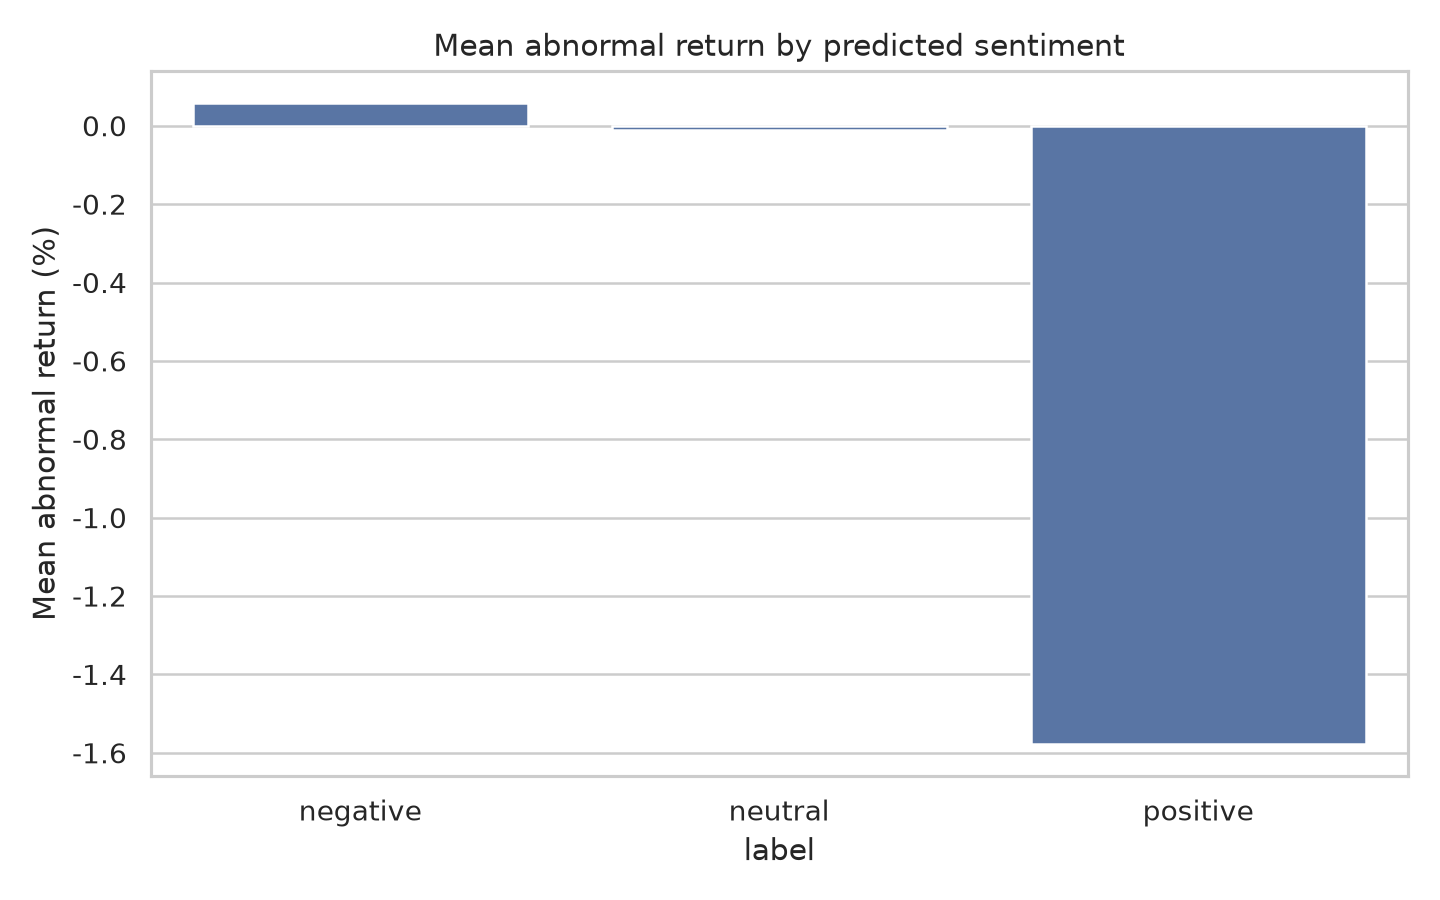
\includegraphics[width=\linewidth]{2019-10/analysis/figures/abnormal_return_by_label.png}
\caption{October 2019}
\end{subfigure}
\begin{subfigure}[t]{0.47\textwidth}
\centering
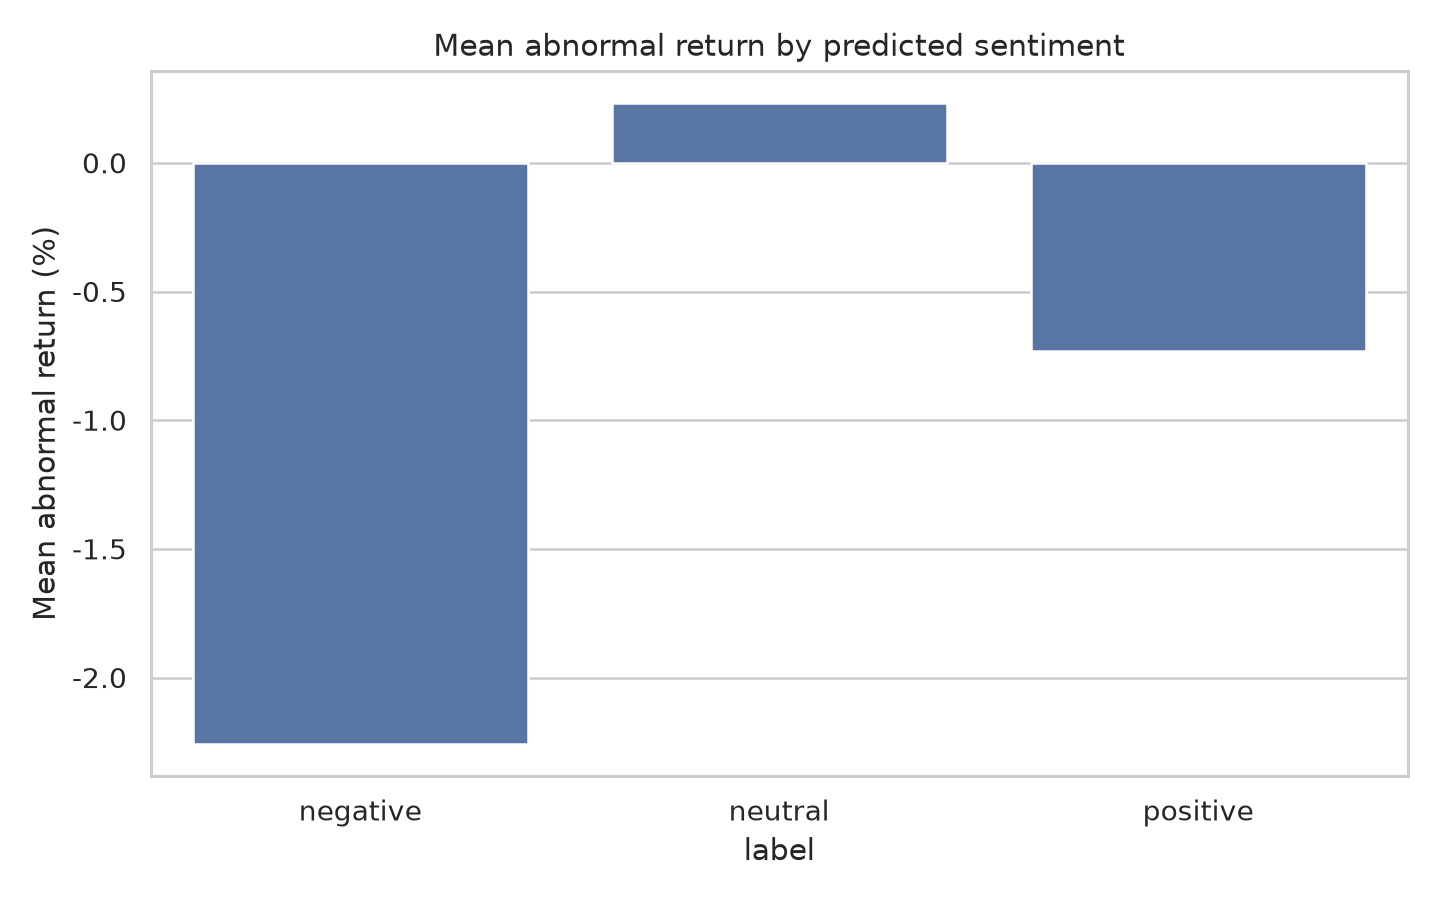
\includegraphics[width=\linewidth]{2020-10/analysis/figures/abnormal_return_by_label.png}
\caption{October 2020}
\end{subfigure}
\begin{subfigure}[t]{0.47\textwidth}
\centering
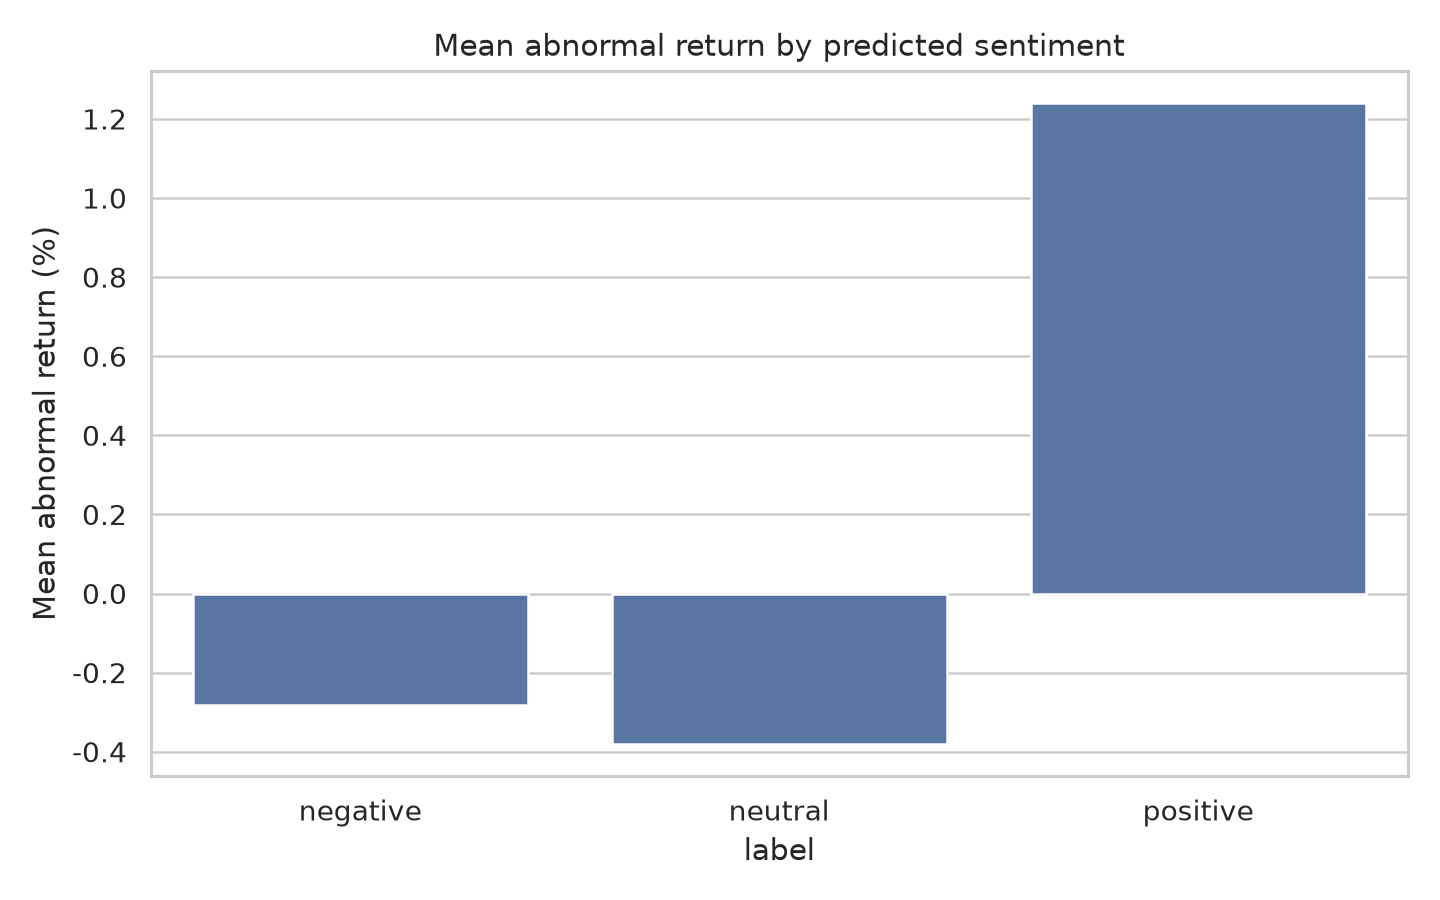
\includegraphics[width=\linewidth]{2021-10/analysis/figures/abnormal_return_by_label.png}
\caption{October 2021}
\end{subfigure}
\begin{subfigure}[t]{0.47\textwidth}
\centering
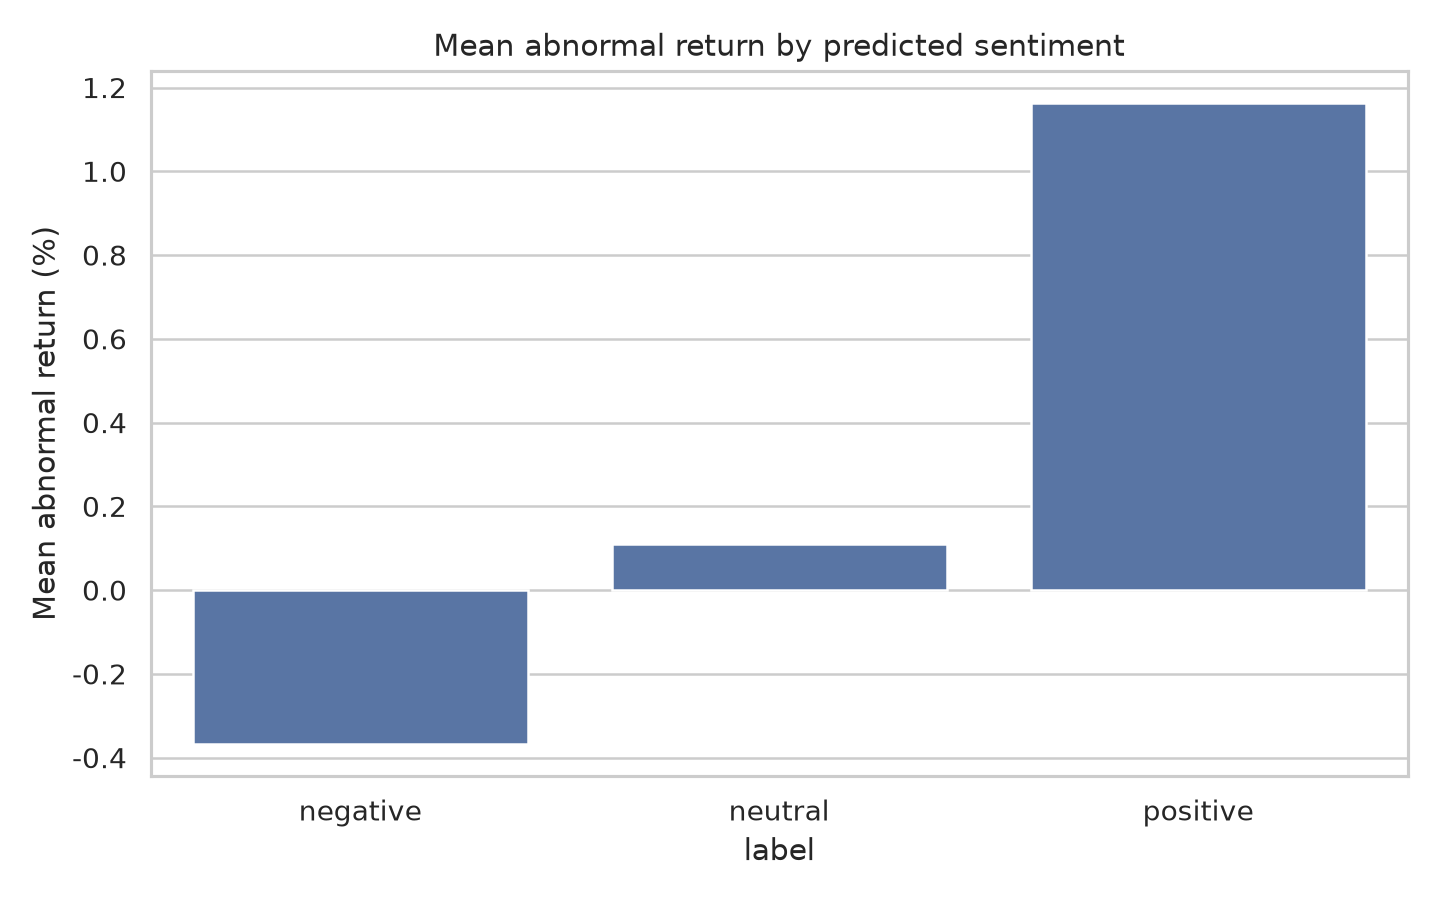
\includegraphics[width=\linewidth]{2022-10/analysis/figures/abnormal_return_by_label.png}
\caption{October 2022}
\end{subfigure}
\caption{Period-specific abnormal-return distributions by predicted sentiment label. The four panels use the same plotting convention and show why sentiment-group estimates must be interpreted together with sample size and uncertainty.}
\label{fig:period-abnormal-return-by-label}
\end{figure}

\paragraph{Market data.}
Daily OHLCV data were retrieved through \texttt{vnstock} for the identified securities and the VNINDEX and VN30 reference series. For every October period, the stored price window begins in May of the same year and ends in December. This provides pre-event observations for the market model and post-event observations for lag calculations without importing prices from a different calendar regime.

\begin{table}[htbp]
\centering
\small
\caption{Market-price coverage by October period.}
\label{tab:multi-year-price-coverage}
\begin{tabular}{lrrrrr}
\toprule
\textbf{Period} & \textbf{Price rows} & \textbf{Symbols} & \textbf{Price start} & \textbf{Price end} & \textbf{Strict rows with price} \\
\midrule
October 2019 & 8,320 & 49 & 2019-05-02 & 2019-12-31 & 141 \\
October 2020 & 9,449 & 57 & 2020-05-04 & 2020-12-31 & 168 \\
October 2021 & 11,935 & 73 & 2021-05-04 & 2021-12-31 & 281 \\
October 2022 & 9,182 & 55 & 2022-05-04 & 2022-12-30 & 206 \\
\bottomrule
\end{tabular}
\end{table}

The number of symbols differs by period because the news corpus and entity-linking output differ across years. The price data are therefore comparable in construction, but not identical in cross-sectional composition. This point is important when comparing the magnitude of estimates across periods.

\subsection{Time Alignment and Return Construction}
\label{subsec:time-alignment-multi-year}

The data contain daily prices but not the exact time at which an article was disseminated to market participants. The implemented alignment rule maps each article's normalized publication date to the first trading date strictly after that calendar date. Thus, an article published on a trading day is evaluated against the next available trading session; an article published on a weekend or holiday is also mapped to the next trading session. No fixed 15:00 cutoff is imposed, because the daily data do not identify the intraday time at which the information was incorporated into the price.

For security $i$ on trading date $t$, the continuously compounded percentage return is computed as
\begin{equation}
 r_{i,t}=100\times\left[\log(P_{i,t})-\log(P_{i,t-1})\right],
\end{equation}
where $P_{i,t}$ is the recorded closing price. The market return is computed using the same transformation for VNINDEX. The analysis uses the downloaded price series as stored; any interpretation of return magnitude is conditional on the source's adjustment and corporate-action coverage.

The sentiment score is a deterministic label encoding:
\begin{equation}
 S_{i,t}=\begin{cases}
 +1,&\text{positive prediction},\\
 0,&\text{neutral prediction},\\
 -1,&\text{negative prediction}.
 \end{cases}
\end{equation}

Several article--ticker rows can refer to the same ticker on the same date. Because the market supplies one return observation per ticker--day, the financial unit is formed by aggregation before inference. The panel records mean sentiment, positive/neutral/negative shares, the number of unique articles, and the number of contributing article--ticker rows. This avoids artificially multiplying the effective sample size by repeating one return for every article.

\subsection{Event-Study Methodology}
\label{subsec:event-study-multi-year}

Following the standard market-model event-study framework of Brown and Warner~\cite{brownwarner1985}, the expected return for each security is estimated from observations before 1 October of the relevant year:
\begin{equation}
 R_{i,t}=\alpha_i+\beta_iR_{m,t}+\varepsilon_{i,t},
\end{equation}
where $R_{m,t}$ is the VNINDEX return. The abnormal return is
\begin{equation}
 AR_{i,t}=R_{i,t}-\left(\widehat{\alpha}_i+\widehat{\beta}_iR_{m,t}\right).
\end{equation}
A security-specific market model is fitted when at least 20 pre-event observations are available; otherwise the documented fallback parameters are retained. The final period-specific runs contain 49, 57, 73, and 55 stored price symbols, respectively, with 54 fitted market-model records in the October 2022 run and corresponding period-specific records in the other runs.

For an event aligned to trading date $t$, cumulative abnormal return is defined as
\begin{equation}
 CAR_i(T_1,T_2)=\sum_{\tau=T_1}^{T_2}AR_{i,t+\tau}.
\end{equation}
Three windows are examined: $[0,0]$ for the event session, $[0,+1]$ for the event session and the next session, and $[0,+3]$ for the event session and the next three sessions. For every period and window, the pipeline reports the mean and median CAR, a two-sided one-sample $t$-test against zero, a two-sided sign-flip permutation test with 5,000 replications, and a percentile bootstrap 95\% confidence interval with 5,000 replications. Fixed random seeds make the resampling results reproducible.



\begin{longtable}{llrrrrrr}
\caption{Aggregate event-study CAR tests by period and event window.}\label{tab:multi-year-car-tests}\\
\toprule
\textbf{Period} & \textbf{Window} & \textbf{N} & \textbf{Mean} & \textbf{Median} & \textbf{$p_t$} & \textbf{$p_{perm}$} & \textbf{Bootstrap 95\% CI} \\
\midrule
\endfirsthead
\toprule
\textbf{Period} & \textbf{Window} & \textbf{N} & \textbf{Mean} & \textbf{Median} & \textbf{$p_t$} & \textbf{$p_{perm}$} & \textbf{Bootstrap 95\% CI} \\
\midrule
\endhead
\midrule
\multicolumn{8}{r}{Continued on next page}\\
\endfoot
\bottomrule
\endlastfoot
2019-10 & $[0,0]$ & 120 & -0.1323 & -0.1570 & 0.5420 & 0.5491 & $[-0.5550,0.2916]$ \\
2019-10 & $[0,+1]$ & 120 & 0.0573 & -0.1285 & 0.8833 & 0.8830 & $[-0.6841,0.8108]$ \\
2019-10 & $[0,+3]$ & 120 & 0.0020 & -0.2812 & 0.9970 & 0.9974 & $[-1.0491,1.0923]$ \\
2020-10 & $[0,0]$ & 134 & 0.0522 & -0.2528 & 0.8031 & 0.8072 & $[-0.3645,0.4595]$ \\
2020-10 & $[0,+1]$ & 134 & -0.2975 & -0.6585 & 0.3424 & 0.3363 & $[-0.8991,0.3050]$ \\
2020-10 & $[0,+3]$ & 133 & -0.9261 & -1.3113 & 0.0438 & 0.0440 & $[-1.8254,-0.0657]$ \\
2021-10 & $[0,0]$ & 212 & -0.2797 & -0.4321 & 0.1070 & 0.1096 & $[-0.6117,0.0587]$ \\
2021-10 & $[0,+1]$ & 212 & -0.2584 & -0.5174 & 0.2920 & 0.2953 & $[-0.7377,0.2377]$ \\
2021-10 & $[0,+3]$ & 212 & -1.0149 & -1.0412 & 0.0101 & 0.0088 & $[-1.7967,-0.2662]$ \\
2022-10 & $[0,0]$ & 150 & 0.1363 & 0.0008 & 0.6023 & 0.6091 & $[-0.3557,0.6421]$ \\
2022-10 & $[0,+1]$ & 150 & -0.0220 & 0.1798 & 0.9501 & 0.9562 & $[-0.7298,0.6360]$ \\
2022-10 & $[0,+3]$ & 150 & -0.2889 & -0.7977 & 0.5614 & 0.5615 & $[-1.2725,0.6793]$ \\
\end{longtable}

\paragraph{Event-study results.}
The aggregate CAR results do not support a single stable sentiment-linked price response across the four October periods. The same-day window is statistically indistinguishable from zero in every period: all $p$-values exceed 0.10 and all bootstrap intervals include zero. In the three-session window, 2020-10 and 2021-10 produce negative mean CAR estimates with nominal $p$-values below 0.05. These two results are noteworthy but should not be treated as decisive evidence: they are two findings among many period--window tests, they are not adjusted for multiple comparisons, and the negative three-session CAR is not itself evidence that sentiment caused the decline.

The 2019 and 2022 estimates remain close to zero or statistically imprecise across all windows. This cross-period heterogeneity is more consistent with a period-dependent market association than with a universal FinABSA effect. It may reflect differences in market regime, news composition, entity coverage, macroeconomic shocks, or the composition of the available price universe.

\subsection{News-Day Versus No-News-Day Control}
\label{subsec:news-control-multi-year}

The event study is complemented by a control comparison. For each period, the control sample contains eligible ticker--days belonging to tickers that appear in the event sample, restricted to October of that year. A news ticker--day is a ticker--day with at least one aligned article event; a no-news ticker--day is an eligible ticker--day without an identified event. The estimand is
\begin{equation}
 \Delta=\overline{AR}_{news}-\overline{AR}_{no\text{-}news}.
\end{equation}

The two distributions are compared using a Welch unequal-variance test, a pooled-label permutation test with 5,000 permutations, and a percentile bootstrap interval for the difference in means.

\begin{table}[htbp]
\centering
\scriptsize
\caption{News-day versus eligible no-news-day abnormal returns.}
\label{tab:news-control-multi-year}
\begin{tabular}{lrrrrrrrr}
\toprule
\textbf{Period} & \textbf{$N_{news}$} & \textbf{$N_{0}$} & \textbf{News mean} & \textbf{No-news mean} & \textbf{$\Delta$} & \textbf{Welch $p$} & \textbf{Perm. $p$} & \textbf{Bootstrap 95\% CI} \\
\midrule
2019-10 & 120 & 941 & -0.1323 & 0.0064 & -0.1386 & 0.5383 & 0.4585 & $[-0.5937,0.3095]$ \\
2020-10 & 134 & 1,027 & 0.0522 & -0.2161 & 0.2683 & 0.2240 & 0.1828 & $[-0.1601,0.7062]$ \\
2021-10 & 212 & 1,217 & -0.2797 & -0.1039 & -0.1758 & 0.3553 & 0.3771 & $[-0.5493,0.1980]$ \\
2022-10 & 150 & 936 & 0.1363 & -0.3559 & 0.4921 & 0.0804 & 0.0684 & $[-0.0645,1.0442]$ \\
\bottomrule
\end{tabular}
\end{table}



The control comparison does not reject equality at the 5\% level in any period. The largest positive point estimate occurs in October 2022, where news days have 0.4921 percentage points higher abnormal returns than no-news days, but the Welch and permutation $p$-values are 0.0804 and 0.0684, respectively, and the bootstrap interval crosses zero. The result is therefore suggestive but not conventionally significant. The comparison remains observational because news selection is not random: firms that receive coverage may systematically differ from firms that do not.

\subsection{Sentiment-Group Contrasts}
\label{subsec:sentiment-groups-multi-year}

At the ticker--day level, the analysis compares three pre-specified contrasts: positive minus neutral, negative minus neutral, and positive minus negative. Each contrast is evaluated with a Welch test, a pooled permutation test, and a bootstrap interval. Differences are defined as group A minus group B.

\begin{longtable}{llrrrrrr}
\caption{Sentiment-group abnormal-return contrasts by period.}\label{tab:sentiment-contrasts-multi-year}\\
\toprule
\textbf{Period} & \textbf{Contrast} & \textbf{$N_A$} & \textbf{$N_B$} & \textbf{Difference} & \textbf{Welch $p$} & \textbf{Perm. $p$} & \textbf{Bootstrap 95\% CI} \\
\midrule
\endfirsthead
\toprule
\textbf{Period} & \textbf{Contrast} & \textbf{$N_A$} & \textbf{$N_B$} & \textbf{Difference} & \textbf{Welch $p$} & \textbf{Perm. $p$} & \textbf{Bootstrap 95\% CI} \\
\midrule
\endhead
\midrule
\multicolumn{8}{r}{Continued on next page}\\
\endfoot
\bottomrule
\endlastfoot
2019-10 & Positive $-$ Neutral & 6 & 113 & -1.5118 & 0.1196 & 0.1252 & $[-3.2365,-0.3238]$ \\
2019-10 & Negative $-$ Neutral & 1 & 113 & -- & -- & -- & Not estimable \\
2019-10 & Positive $-$ Negative & 6 & 1 & -- & -- & -- & Not estimable \\
2020-10 & Positive $-$ Neutral & 10 & 123 & -0.8544 & 0.3380 & 0.2813 & $[-2.1566,0.9352]$ \\
2020-10 & Negative $-$ Neutral & 1 & 123 & -- & -- & -- & Not estimable \\
2020-10 & Positive $-$ Negative & 10 & 1 & -- & -- & -- & Not estimable \\
2021-10 & Positive $-$ Neutral & 12 & 191 & 1.5693 & 0.0267 & 0.0388 & $[0.5210,2.8516]$ \\
2021-10 & Negative $-$ Neutral & 9 & 191 & 0.0915 & 0.9093 & 0.9112 & $[-1.0946,1.7607]$ \\
2021-10 & Positive $-$ Negative & 12 & 9 & 1.4779 & 0.1460 & 0.1372 & $[-0.4072,3.2104]$ \\
2022-10 & Positive $-$ Neutral & 14 & 126 & 0.6990 & 0.4518 & 0.4271 & $[-0.9308,2.4970]$ \\
2022-10 & Negative $-$ Neutral & 10 & 126 & -0.4688 & 0.6712 & 0.6601 & $[-2.5243,1.4876]$ \\
2022-10 & Positive $-$ Negative & 14 & 10 & 1.1678 & 0.3962 & 0.3971 & $[-1.2938,3.6937]$ \\
\end{longtable}

The most notable group contrast appears in October 2021: the positive group has a 1.5693 percentage-point higher mean abnormal return than the neutral group, with Welch $p=0.0267$, permutation $p=0.0388$, and a bootstrap interval that excludes zero. This result should be described as a period-specific exploratory finding rather than a general law. The positive group contains only 12 ticker--day observations, the negative group contains nine, the analysis involves multiple comparisons, and the effect is not replicated in the corresponding positive--neutral comparisons for 2019, 2020, or 2022.

The 2019 positive--neutral point estimate is negative, whereas the 2020 and 2022 differences are also statistically imprecise. The failure of sign consistency across years weakens the claim that predicted sentiment produces a stable cross-sectional ranking of abnormal returns.



\subsection{Two-Way Fixed-Effects Panel Regression}
\label{subsec:panel-regression-multi-year}

To control for persistent differences between securities and common shocks across dates, the following two-way fixed-effects model is estimated separately for each October period:
\begin{equation}
 AR_{i,\tau(i,t)}=\alpha_i+\delta_{\tau(i,t)}+\beta_1S_{i,t}
 +\beta_2\mathrm{NegativeShare}_{i,t}
 +\beta_3\mathrm{PositiveShare}_{i,t}
 +\gamma\log(1+\mathrm{ArticleCount}_{i,t})+\varepsilon_{i,t},
\end{equation}
where $\alpha_i$ denotes ticker fixed effects, $\delta_{\tau(i,t)}$ denotes date fixed effects, and $\tau(i,t)$ is the first trading session strictly after publication. The dependent variable is market-model abnormal return on the aligned evaluation date.

\begin{table}[htbp]
\centering
\scriptsize
\caption{Key coefficients from period-specific two-way fixed-effects regressions. The full coefficient tables, including ticker and date fixed-effect indicators, are provided in the accompanying CSV output.}
\label{tab:panel-key-coefficients-multi-year}
\begin{tabular}{llrrrr}
\toprule
\textbf{Period} & \textbf{Variable} & \textbf{Coefficient} & \textbf{Std. error} & \textbf{$t$-statistic} & \textbf{$p$-value} \\
\midrule
2019-10 & Sentiment score & -0.4450 & 0.8508 & -0.5230 & 0.6009 \\
2019-10 & Negative share & 1.5084 & 1.8412 & 0.8192 & 0.4127 \\
2019-10 & Positive share & 1.0633 & 1.2562 & 0.8468 & 0.3973 \\
2019-10 & Log article count & -1.5405 & 3.3930 & -0.4540 & 0.6498 \\
2020-10 & Sentiment score & 2.5056 & 0.8042 & 3.1156 & 0.0018 \\
2020-10 & Negative share & -4.9332 & 1.8033 & -2.7356 & 0.0062 \\
2020-10 & Positive share & -2.4276 & 1.2770 & -1.9010 & 0.0573 \\
2020-10 & Log article count & 2.3897 & 1.9986 & 1.1957 & 0.2318 \\
2021-10 & Sentiment score & -0.9696 & 2.4681 & -0.3927 & 0.6944 \\
2021-10 & Negative share & 0.1799 & 2.5174 & 0.0715 & 0.9430 \\
2021-10 & Positive share & 0.4345 & 2.6128 & 0.1663 & 0.8679 \\
2021-10 & Log article count & 0.5867 & 1.0124 & 0.5795 & 0.5623 \\
2022-10 & Sentiment score & 6.5062 & 5.3763 & 1.2100 & 0.2262 \\
2022-10 & Negative share & 5.9827 & 5.2919 & 1.1305 & 0.2582 \\
2022-10 & Positive share & -6.1476 & 5.5086 & -1.1160 & 0.2644 \\
2022-10 & Log article count & 0.3079 & 1.3849 & 0.2224 & 0.8241 \\
\bottomrule
\end{tabular}
\end{table}

The sentiment-score coefficient is positive and statistically significant only in the 2020 period. The coefficient is negative and insignificant in 2019 and 2021, and positive but imprecise in 2022. This sign instability is central: a robust sentiment--return association would be expected to exhibit a more consistent direction under comparable definitions. The 2020 coefficient therefore constitutes a period-specific association, not evidence that the model has a stable return-prediction relationship.

The coefficient on negative share is also significant only in 2020 and is negative, while the positive-share coefficient is not significant at the 5\% level. Because sentiment shares are compositional and mechanically related to the omitted neutral share, their coefficients should not be interpreted as independent causal marginal effects. The relatively high within-period $R^2$ values are not evidence of strong predictive power: ticker and date fixed effects can absorb substantial variation, while the sentiment covariates remain sensitive to sample composition.

The intended covariance estimator was HC3. In sparse two-way fixed-effects designs, HC3 can produce infinite standard errors when leverage reaches a singular boundary. The implementation therefore falls back to HC1 when necessary and records this fallback in the period-specific metadata. These panel coefficients should consequently be treated as exploratory conditional associations.



\subsection{Lagged Robustness and Sensitivity Analysis}
\label{subsec:lag-robustness-multi-year}

Lag analysis evaluates abnormal returns at 0, 1, 2, 3, 5, and 10 trading sessions after the aligned event date. These are sensitivity checks rather than independent causal tests. The sample size decreases at longer lags because the relevant security price must remain available after the event.

\begin{longtable}{llrrrrrr}
\caption{Lagged abnormal-return robustness by period.}\label{tab:lag-robustness-multi-year}\\
\toprule
\textbf{Period} & \textbf{Lag} & \textbf{N} & \textbf{Overall AR} & \textbf{Negative} & \textbf{Neutral} & \textbf{Positive} \\
\midrule
\endfirsthead
\toprule
\textbf{Period} & \textbf{Lag} & \textbf{N} & \textbf{Overall AR} & \textbf{Negative} & \textbf{Neutral} & \textbf{Positive} \\
\midrule
\endhead
\midrule
\multicolumn{7}{r}{Continued on next page}\\
\endfoot
\bottomrule
\endlastfoot
2019-10 & 0 & 120 & -0.1323 & -1.5766 & -0.0648 & 0.8940 \\
2019-10 & 1 & 146 & 0.3194 & 0.0588 & 0.2772 & 1.2785 \\
2019-10 & 2 & 141 & -0.0968 & 0.0331 & -0.0974 & -0.1286 \\
2019-10 & 3 & 134 & 0.0067 & -0.4507 & 0.0283 & -0.3248 \\
2019-10 & 5 & 108 & 0.1154 & -0.6470 & 0.1166 & 0.2232 \\
2019-10 & 10 & 74 & -0.1635 & 0.1766 & -0.1547 & -0.6273 \\
2020-10 & 0 & 134 & 0.2261 & -1.9519 & 0.3085 & -0.4498 \\
2020-10 & 1 & 164 & -0.1520 & 0.5470 & -0.1975 & 0.2915 \\
2020-10 & 2 & 159 & -0.3772 & 1.3165 & -0.3780 & -0.7051 \\
2020-10 & 3 & 152 & 0.0687 & 0.9315 & 0.1112 & -0.6345 \\
2020-10 & 5 & 144 & -0.0997 & 0.4069 & -0.1472 & 0.4869 \\
2020-10 & 10 & 100 & -0.4924 & 0.3574 & -0.5596 & 1.5471 \\
2021-10 & 0 & 212 & -0.0285 & -0.1815 & -0.0939 & 1.0708 \\
2021-10 & 1 & 267 & 0.2065 & 0.6397 & 0.2368 & -0.5095 \\
2021-10 & 2 & 255 & -0.3156 & -0.4267 & -0.2764 & -0.8200 \\
2021-10 & 3 & 244 & 0.0773 & -0.3897 & 0.1940 & -1.2377 \\
2021-10 & 5 & 219 & 0.1398 & -0.1027 & 0.1966 & -0.4387 \\
2021-10 & 10 & 147 & -0.0471 & 1.2318 & -0.1101 & -0.1871 \\
2022-10 & 0 & 150 & -0.0936 & -0.7884 & -0.1653 & 0.8940 \\
2022-10 & 1 & 174 & -0.1797 & 0.3368 & 0.0713 & -2.7331 \\
2022-10 & 2 & 163 & -0.2007 & -1.2344 & -0.0991 & -0.4067 \\
2022-10 & 3 & 153 & -0.5972 & -2.6554 & -0.4837 & -0.1760 \\
2022-10 & 5 & 134 & -0.7243 & 0.4479 & -0.9416 & 0.5251 \\
2022-10 & 10 & 93 & -0.5183 & -0.4422 & -0.2779 & -4.1530 \\
\end{longtable}



The lag results do not display a common monotonic decay. In 2019, the overall estimate changes from negative at lag 0 to positive at lag 1 and back toward zero thereafter. In 2020, the estimates become more negative at lags 2 and 10, while in 2021 the sign alternates across horizons. In 2022, the overall mean is increasingly negative at lags 3 and 5. Sentiment-specific estimates are even less stable, particularly for the small positive and negative groups. The appropriate conclusion is that the apparent price association depends on the timing convention and the available evaluation horizon.

\subsection{Additional Diagnostic Evidence}
\label{subsec:additional-diagnostics-multi-year}

The output package also contains daily ticker--day sentiment and abnormal-return tables, market-model coverage, event observations, and panel-regression data. These artifacts support auditability and allow the reader to trace each reported result back to an aligned ticker--day observation. The following diagnostic figures are descriptive rather than inferential.

\begin{figure}[htbp]
\centering
\begin{subfigure}[t]{0.47\textwidth}
\centering
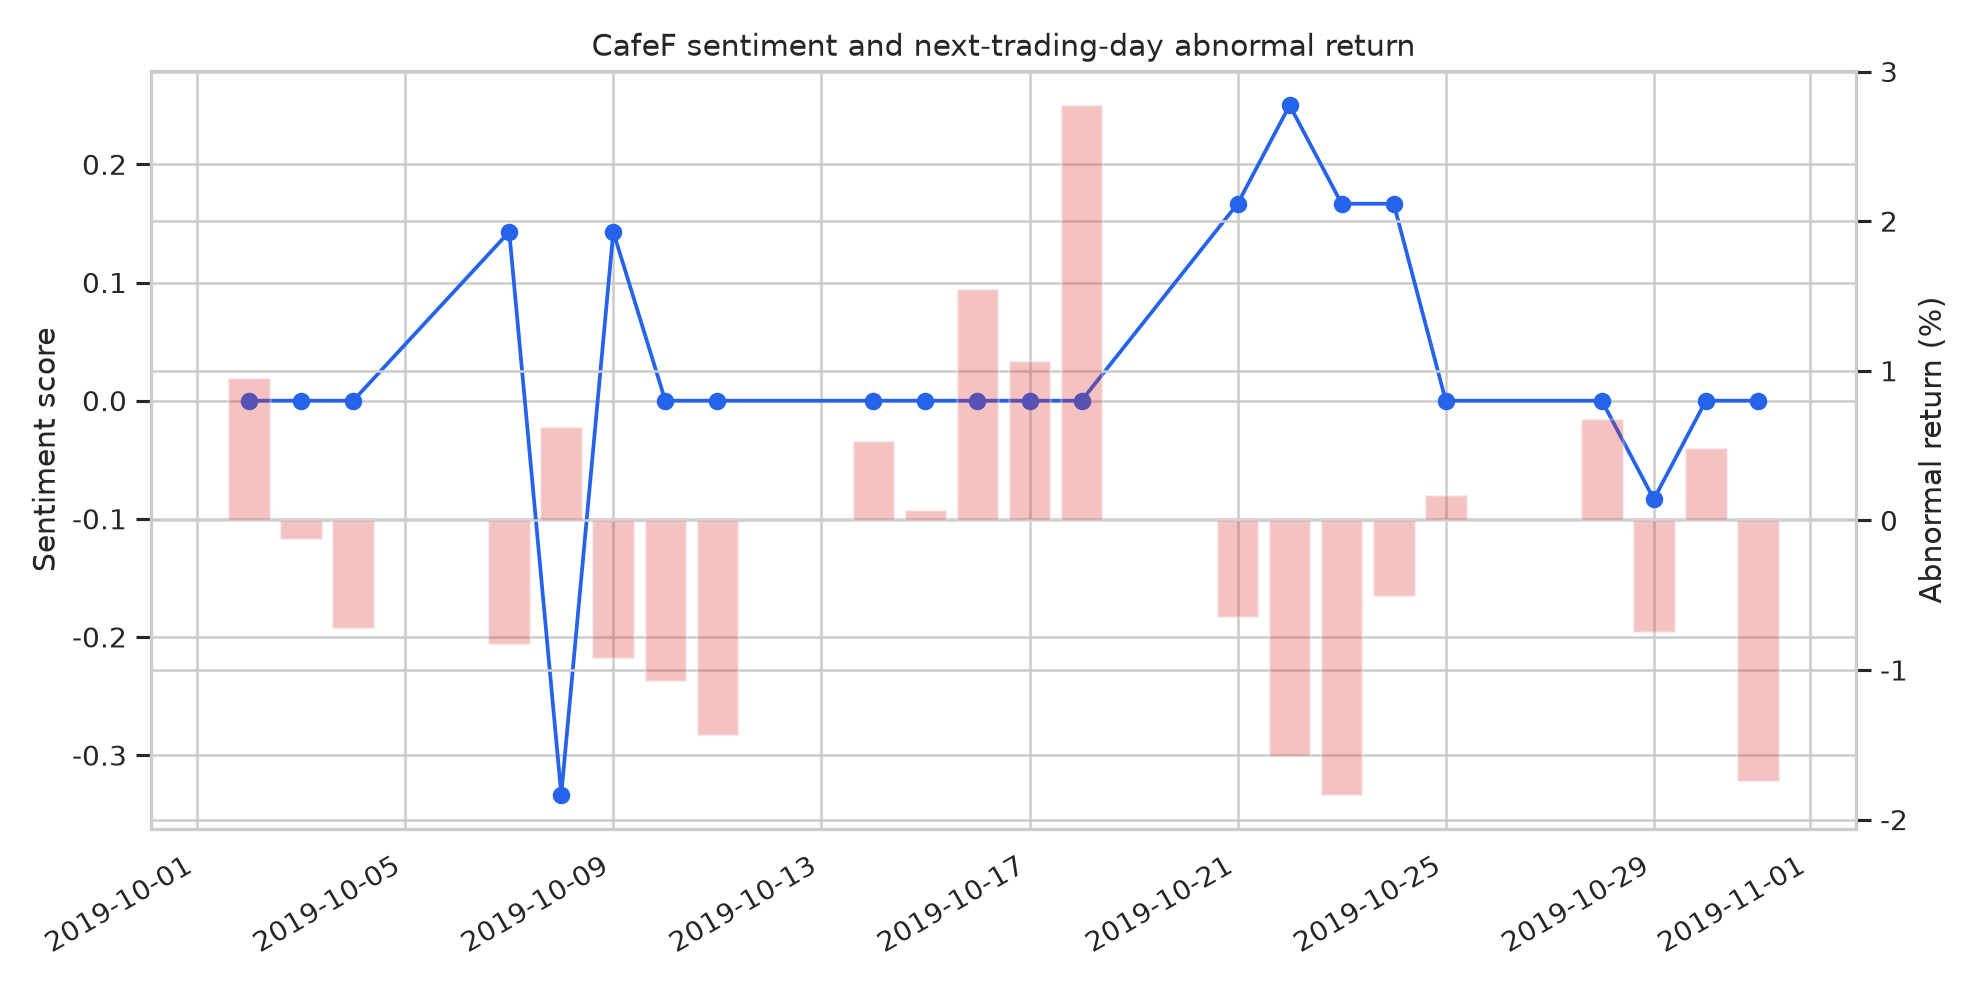
\includegraphics[width=\linewidth]{2019-10/analysis/figures/sentiment_vs_abnormal_return.png}
\caption{October 2019}
\end{subfigure}
\begin{subfigure}[t]{0.47\textwidth}
\centering
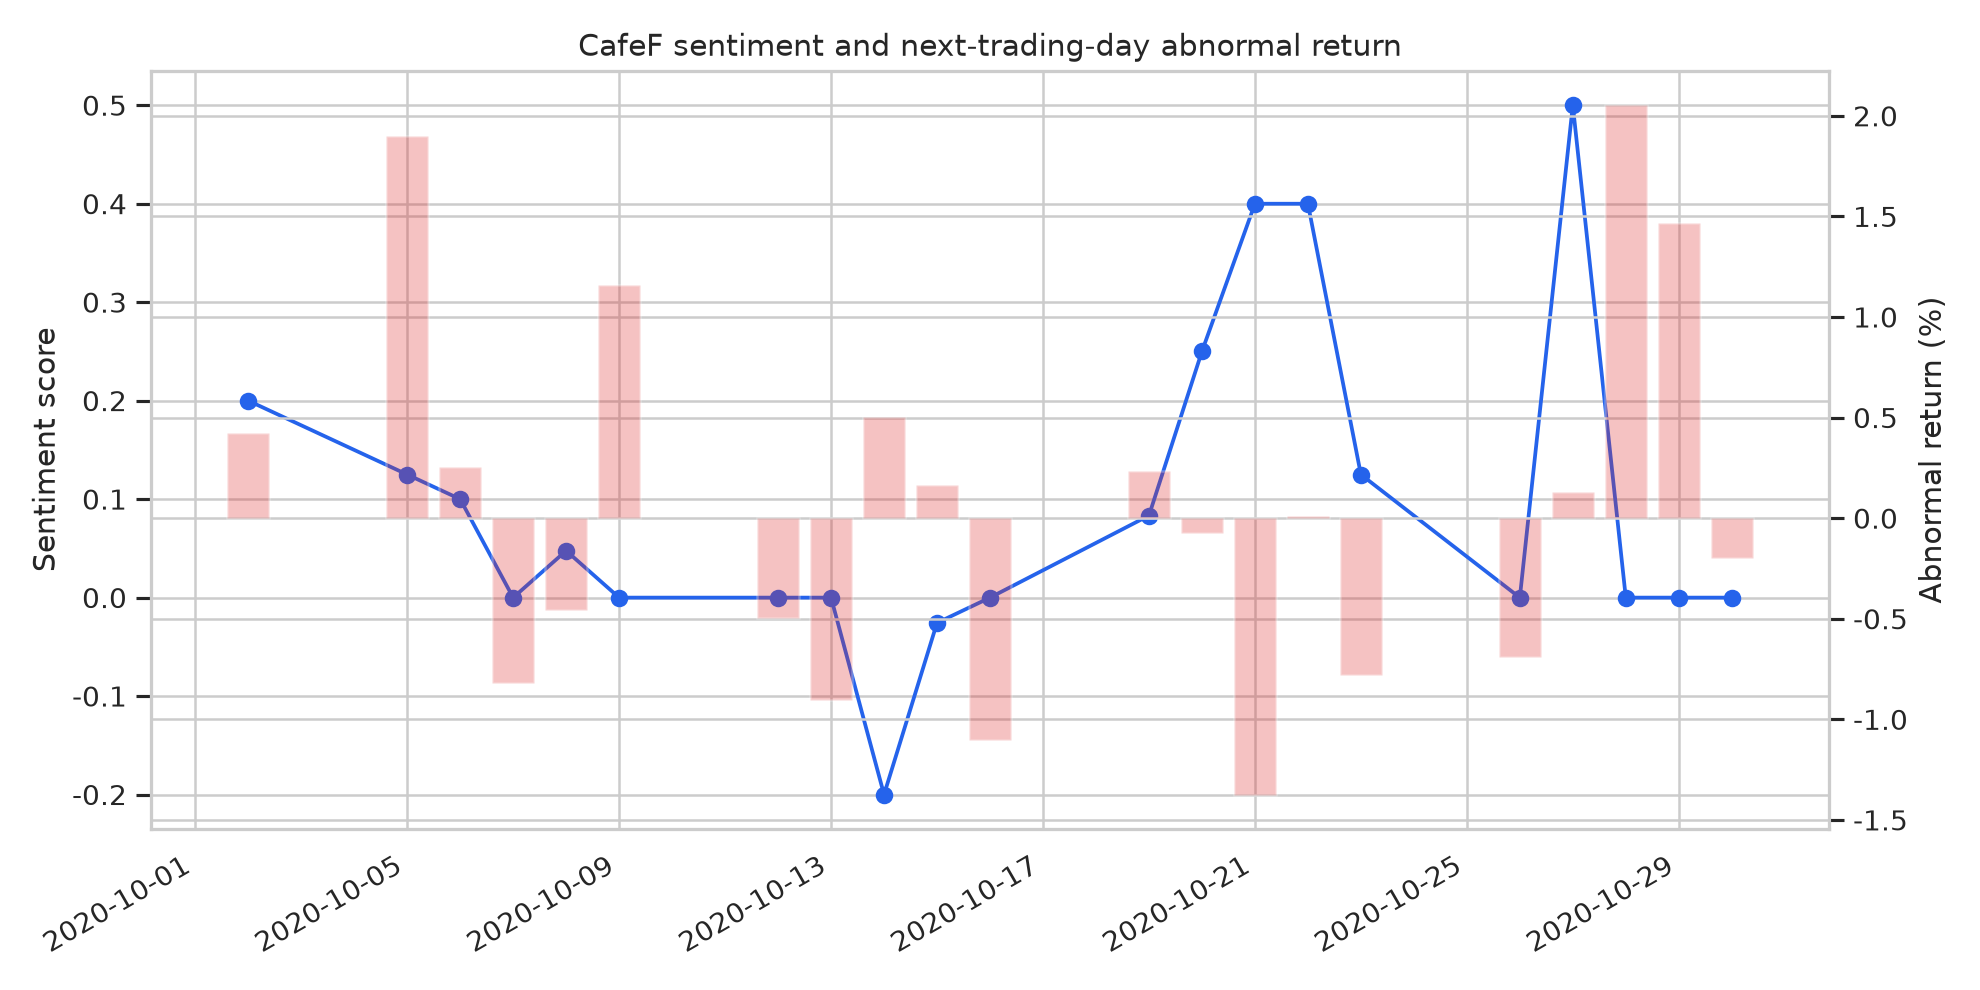
\includegraphics[width=\linewidth]{2020-10/analysis/figures/sentiment_vs_abnormal_return.png}
\caption{October 2020}
\end{subfigure}
\begin{subfigure}[t]{0.47\textwidth}
\centering
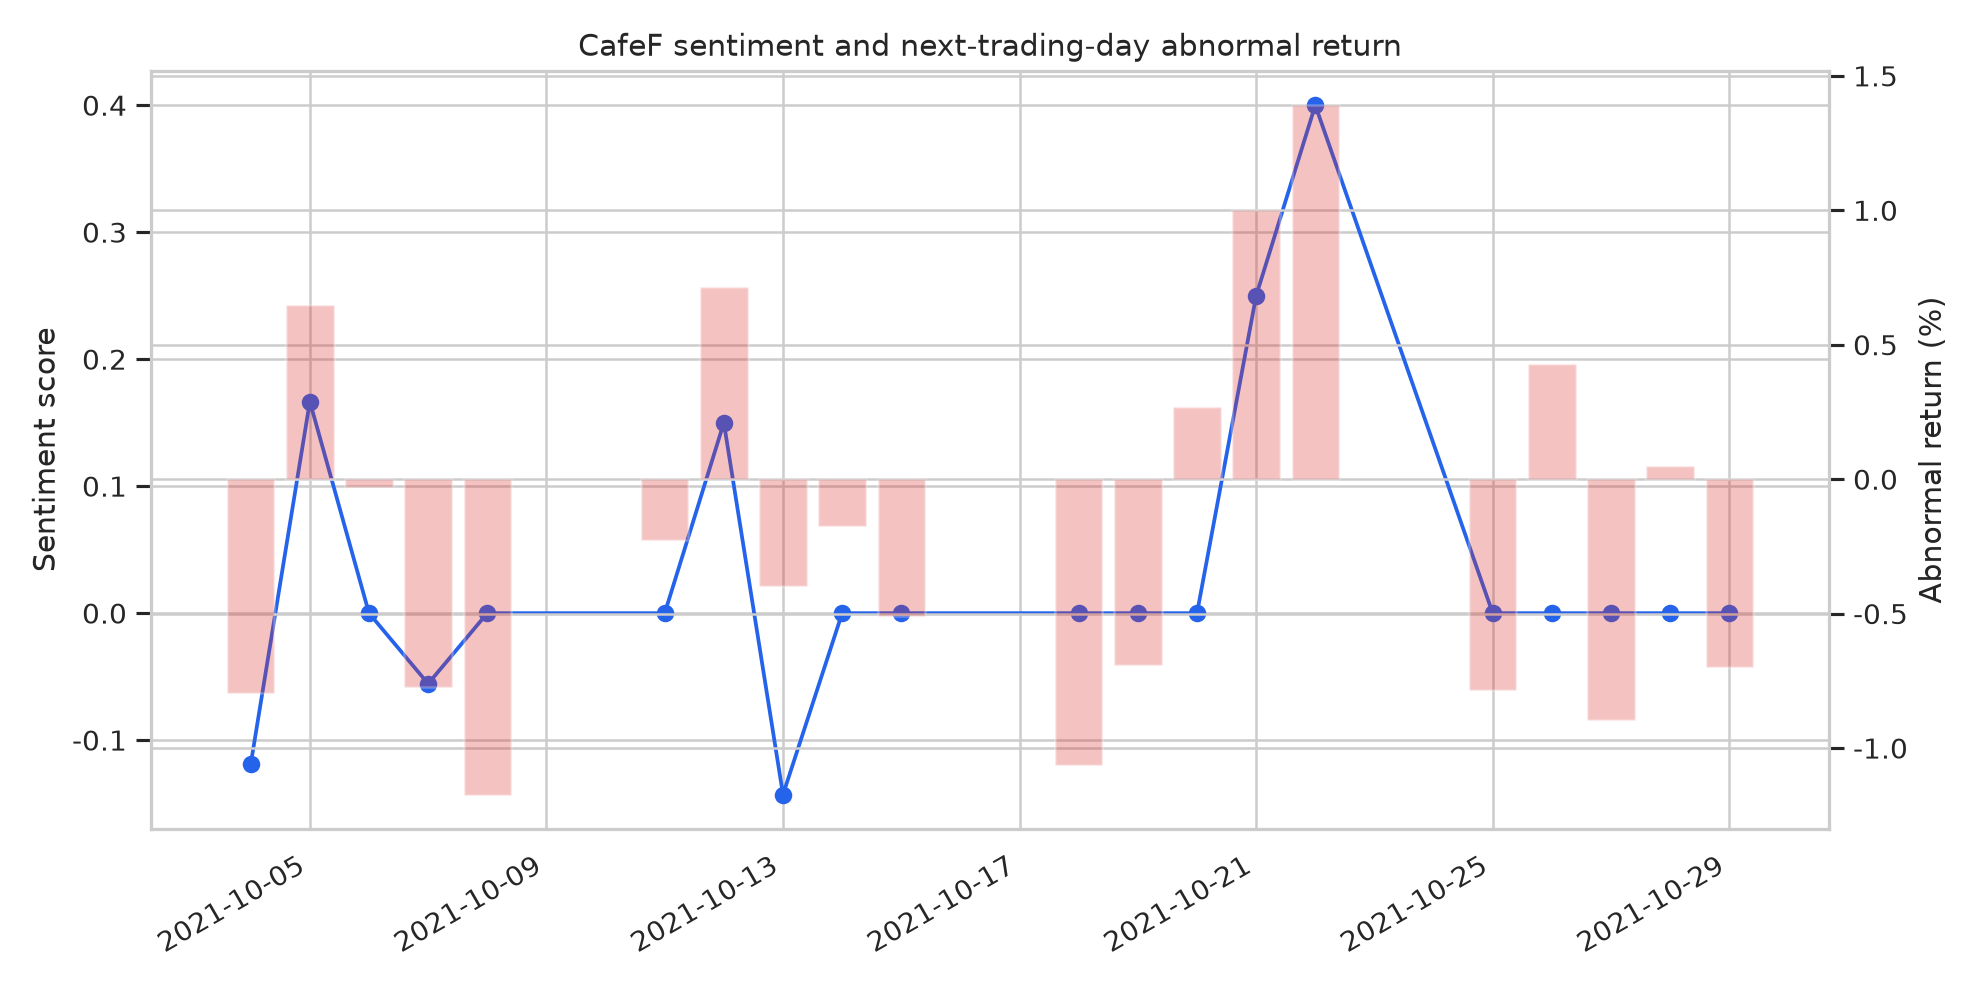
\includegraphics[width=\linewidth]{2021-10/analysis/figures/sentiment_vs_abnormal_return.png}
\caption{October 2021}
\end{subfigure}
\begin{subfigure}[t]{0.47\textwidth}
\centering
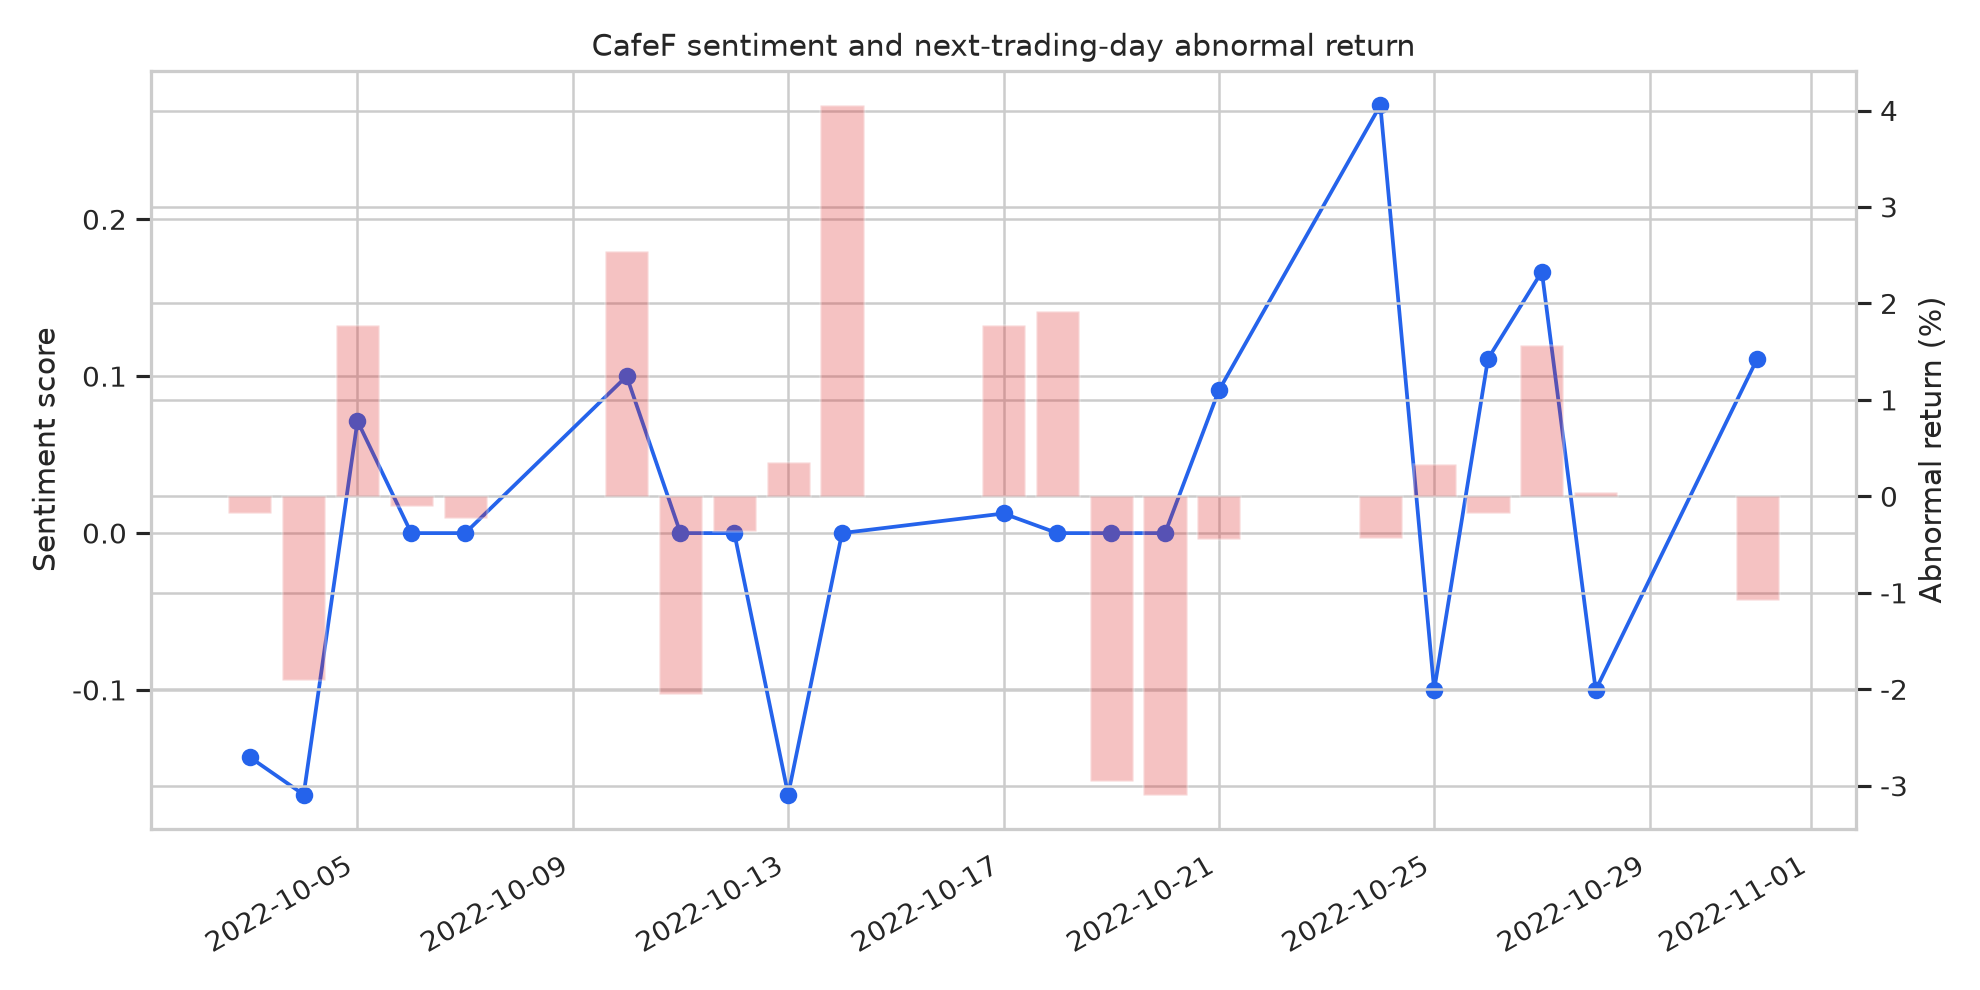
\includegraphics[width=\linewidth]{2022-10/analysis/figures/sentiment_vs_abnormal_return.png}
\caption{October 2022}
\end{subfigure}
\caption{Period-specific descriptive comparisons between daily mean sentiment and mean abnormal return. These panels are descriptive diagnostics, not causal identification plots.}
\label{fig:period-sentiment-vs-abnormal-return}
\end{figure}

\subsection{Multiple Comparisons and Statistical Interpretation}
\label{subsec:multiple-comparisons}

The multi-year design produces several families of related tests: four periods, three event windows, multiple sentiment groups, a news-day control, panel coefficients, and six lag horizons. Consequently, at least some nominally small $p$-values can occur by chance when many hypotheses are examined. The results are therefore interpreted using three criteria: the size and direction of the estimate, whether the confidence interval excludes zero, and whether the finding is replicated under related specifications or periods.

Under this framework, the 2020 and 2021 three-day CAR findings and the 2021 positive--neutral contrast are interesting signals for further study, but not definitive discoveries. They should be reported with their exact sample sizes, intervals, and unadjusted $p$-values. A confirmatory study should pre-specify a smaller number of primary hypotheses and apply a family-wise or false-discovery-rate correction, such as Holm or Benjamini--Hochberg, depending on the inferential objective.

\subsection{Analyses Not Validly Estimated in the Current Run}
\label{subsec:deferred-analyses-multi-year}

Several analyses appeared in the initial experimental plan but are not assigned numerical claims here because the required artifacts are absent. First, intrinsic CafeF accuracy, macro-F1, MCC, and Cohen's kappa require an independently human-annotated gold-label sample. The model's own predictions cannot serve as their ground truth. Second, probability calibration metrics such as Expected Calibration Error require valid per-class probabilities or logits; the current prediction files contain hard labels and empty probability fields. Third, out-of-time return forecasting requires a pre-specified chronological training, validation, and test design with a fitted return-prediction model; the current pipeline is an event-study association analysis, not a trained forecaster. Fourth, a broad-linking robustness result requires a complete independent inference and financial analysis run on the 2,740-row broad input set; strict and full input files alone are not sufficient.

This separation is methodologically important. It prevents unsupported accuracy, calibration, forecasting, and robustness numbers from being presented as results. The completed outputs can be extended later without changing the core data contract.

\subsection{Limitations}
\label{subsec:limitations-statistical}

The empirical design is deliberately transparent, but several limitations constrain the strength and generality of the conclusions.

\paragraph{Limited temporal coverage and regime dependence.}
The expanded corpus contains one October sample for each year from 2019 to 2022. This common-month design improves cross-year comparability, but it does not represent the full calendar year or every stage of the COVID-19 shock. The four samples may differ in macroeconomic conditions, market liquidity, news intensity, and sector composition. The analysis should therefore be read as a comparison of four historical snapshots rather than as a complete estimate of a universal news effect.

\paragraph{Non-random news selection and residual confounding.}
CafeF is a single editorial source, and the publication of a story is not randomly assigned. Firms receiving more coverage may be larger, more liquid, more volatile, or already experiencing information shocks. The news-day versus no-news-day control accounts for an observable event indicator but does not remove this selection mechanism. Other confounders, including earnings announcements, market-wide policy news, sector shocks, liquidity changes, and concurrent disclosures, are not fully controlled in the current specification.

\paragraph{Entity-linking and sample-selection error.}
FinABSA classifies sentiment for a pre-specified target; it does not discover tickers. The upstream entity-linking module can produce false positives when an uppercase abbreviation resembles a ticker and false negatives when a company is mentioned through an unseen alias. The strict confidence threshold of 0.95 reduces false-positive links at the cost of coverage. In the completed data, 43 strict article--ticker rows have no usable price window and 32 price retrieval errors are recorded. These rows are not assigned artificial returns, but their exclusion can still create selection effects.

\paragraph{Classifier uncertainty and class imbalance.}
Among 839 strict predictions, 759 are neutral, 54 are positive, and 26 are negative. The small positive and negative groups make group means and confidence intervals sensitive to individual observations. The current prediction files also contain hard labels rather than calibrated class probabilities. Consequently, classification uncertainty is not propagated into the abnormal-return estimates, and the financial tests cannot distinguish a confident prediction from a marginal one.

\paragraph{Daily timing and return measurement.}
The source data do not provide reliable intraday dissemination timestamps for every article. The implemented rule maps each publication date to the first trading session strictly after that date. This rule is reproducible and avoids assuming an unobserved market-close cutoff, but it can delay an article that was published before the close or miss part of a same-day reaction. Returns are computed from daily closing prices and are therefore unable to identify intraday price discovery. The interpretation also depends on the adjustment and corporate-action treatment of the downloaded OHLCV series.

\paragraph{Sparse fixed-effects panels.}
The period-specific panels contain different numbers of ticker--day observations and trading dates. Two-way fixed effects absorb much of the variation in a short panel and can generate high leverage. HC3 covariance estimation becomes unstable in some specifications; the implementation records an HC1 fallback when HC3 produces non-finite standard errors. This safeguard preserves finite estimates but weakens the case for strong regression inference. The panel results should consequently be treated as exploratory conditional associations.

\paragraph{Multiple comparisons and external validity.}
The study examines four periods, three event windows, several group contrasts, a control comparison, panel coefficients, and six lags. Nominal $p$-values are not automatically adjusted for this family of hypotheses. The 2020 and 2021 three-session CAR findings, the 2021 positive--neutral contrast, and the 2020 sentiment coefficient are therefore best treated as hypothesis-generating signals. They do not establish a replicated effect, causal impact, or profitable trading rule. In addition, the use of currently retrievable listed securities can create survivorship and availability bias when the historical universe is reconstructed.

\subsection{Future Work}
\label{subsec:future-work-statistical}

Future work should convert the present exploratory study into a pre-specified confirmatory evaluation. The first priority is an independent CafeF gold set. Multiple annotators should label article--ticker pairs using written guidelines, disagreements should be adjudicated, and inter-annotator agreement should be reported. The gold set must be separated by article and, where possible, by time period, so that repeated headlines or near-duplicate news cannot leak between training and evaluation. This would enable accuracy, balanced accuracy, macro-F1, MCC, Cohen's kappa, confusion matrices, and a proper qualitative error analysis.

The second priority is uncertainty-aware inference. A frozen checkpoint should produce per-class probabilities or logits for every period. These outputs can support Expected Calibration Error, reliability diagrams, confidence-stratified analysis, and probability-weighted sentiment aggregation. Bootstrap procedures should propagate both sampling uncertainty and classifier uncertainty rather than treating every hard label as equally reliable.

The third priority is broader and more balanced temporal coverage. Additional months before, during, and after the pandemic should be collected under the same data contract. A longer panel would support year, sector, and regime interactions and would reduce the dependence of the conclusions on a single October sample. The broad entity-linking sample should also be run end-to-end as an independent sensitivity analysis, with pre-defined rules for comparing its estimates with the strict sample.

The fourth priority is a stronger financial identification design. Future specifications should pre-register the estimation window, use alternative market-adjustment models such as market-adjusted and multi-factor returns, and report standard errors clustered at an appropriate level. Placebo dates, non-news dates, sector-level decomposition, and tests for concurrent corporate disclosures should be included before examining the final results. Multiple-testing control, such as Holm adjustment for a small confirmatory family or false-discovery-rate control for a wider exploratory family, should be selected in advance.

Finally, return forecasting should be separated from event-study inference. If the objective is prediction, a separate chronological forecasting task should be defined with a censor gap between the information date and the evaluation window. Models should be compared with naive and market baselines using out-of-time RMSE, MAE, rank correlation, and economically meaningful portfolio diagnostics. Any trading simulation would additionally require transaction costs, bid--ask spreads, liquidity constraints, position limits, delisting treatment, and strict protection against look-ahead bias. These steps would determine whether the sentiment signal has economic value beyond statistical association.

\subsection{Overall Assessment and Conclusion}
\label{subsec:conclusion-statistical}

The completed study establishes a reproducible NLP-to-finance validation pipeline across 839 strict article--ticker predictions from October 2019, October 2020, October 2021, and October 2022. The pipeline performs stable prediction alignment, next-trading-session mapping, market-model estimation, CAR analysis, news-day control comparisons, sentiment-group tests, two-way fixed-effects regressions, and lag sensitivity analysis. All prediction files are aligned by stable \texttt{sample\_id}; there are no missing predictions, unexpected IDs, duplicate IDs, or unknown labels after normalization.

The statistical evidence is heterogeneous rather than universal. Same-day aggregate CAR is not statistically different from zero in any period. Negative three-session CAR is nominally significant in 2020 and 2021, the positive--neutral contrast is nominally significant only in 2021, and the sentiment coefficient is nominally significant only in the 2020 panel. These findings are not consistently replicated across years or horizons. The news-day control does not reach the conventional 5\% threshold, and lag estimates change direction and magnitude across periods. The pattern therefore does not support a stable, causal, or reliably predictive sentiment effect on Vietnamese stock returns.

The appropriate contribution is methodological and exploratory. The project demonstrates how target-masked ABSA outputs can be linked to Vietnamese listed securities and evaluated through complementary financial tests without silently converting missing data, parser failures, or hard labels into unsupported evidence. The occasional significant estimates provide useful hypotheses for a larger, independently annotated, probability-aware, and pre-registered study, but they should not be presented as a standalone investment strategy.

\begin{table}[htbp]
\centering
\small
\caption{Reproducibility checklist for the completed multi-year validation.}
\label{tab:reproducibility-multi-year}
\begin{tabular}{p{0.42\textwidth}p{0.46\textwidth}}
\toprule
\textbf{Component} & \textbf{Completed implementation} \\
\midrule
Sampling design & October 2019, October 2020, October 2021, October 2022 \\
Price window & May--December of the same year for every period \\
Prediction alignment & Stable \texttt{sample\_id}; 839/839 matched \\
Label normalization & Canonical positive/neutral/negative; zero unknown labels \\
Entity-linking primary sample & Strict confidence threshold $\geq 0.95$ \\
Event mapping & First trading session strictly after publication date \\
Market adjustment & Security-specific market model with VNINDEX proxy \\
Event windows & $[0,0]$, $[0,+1]$, and $[0,+3]$ \\
Inference tests & One-sample $t$-test, sign-flip permutation, bootstrap CI \\
Control test & News-day versus eligible no-news-day comparison \\
Group tests & Welch, permutation, and bootstrap contrasts \\
Panel model & Ticker/date fixed effects; HC1 fallback documented \\
Lag sensitivity & 0, 1, 2, 3, 5, and 10 trading-session lags \\
Output artifacts & CSV tables, period-specific event files, six multi-year figures, Markdown report, Excel workbook \\
\bottomrule
\end{tabular}
\end{table}

The numerical source files are stored under \texttt{data/cafef\_multiyear/analysis\_multiyear/}. The principal tables are \texttt{car\_primary\_all.csv}, \texttt{news\_day\_control\_tests.csv}, \texttt{sentiment\_group\_tests.csv}, \texttt{panel\_key\_coefficients.csv}, \texttt{robustness\_summary.csv}, and \texttt{prediction\_validation\_clean.csv}. The complete workbook is \texttt{multiyear\_validation\_tables.xlsx}, and the period-specific diagnostics are retained under each period's \texttt{analysis/} directory.

\begin{quote}
This is research and analysis only, not personalized financial advice.
\end{quote}

\bibliographystyle{plain}
\begin{thebibliography}{99}
\bibitem{son2023removing}
Son, G., Lee, H., Kang, N., \& Hahm, M. (2023). Removing non-stationary knowledge from pre-trained language models for entity-level sentiment classification in finance. \textit{arXiv preprint arXiv:2301.03136}.

\bibitem{finbert}
Yang, Y., UY, M. C. S., \& Huang, A. (2020). FinBERT: A pretrained language model for financial communications. \textit{arXiv preprint arXiv:2006.08097}.

\bibitem{entfin-dataset}
Hahm, M., \& Son, G. (2023). SEntFiN 1.0: Entity-level Sentiment Dataset for Finance. \textit{Journal of the Association for Information Science and Technology}. DOI: 10.1002/asi.24634.

\bibitem{nonstationary-knowledge-arxiv}
Son, G., Lee, H., Kang, N., \& Hahm, M. (2023). Removing Non-Stationary Knowledge From Pre-Trained Language Models for Entity-Level Sentiment Classification in Finance. \textit{arXiv:2301.03136}.

\bibitem{aspect-sentiment-quad-prediction}
Zhang, W., Li, X., Deng, Y., Bing, L., \& Lam, W. (2021). Aspect Sentiment Quad Prediction as Paraphrase Generation. \textit{arXiv preprint arXiv:2110.00796}.

\bibitem{tetlock2007}
Tetlock, P. C. (2007). Giving content to investor sentiment: The role of media in the stock market. \textit{The Journal of Finance}, 62(3), 1139--1168.

\bibitem{brownwarner1985}
Brown, S. J., \& Warner, J. B. (1985). Using daily stock returns: The case of event studies. \textit{Journal of Financial Economics}, 14(1), 3--31.

\bibitem{fama1970}
Fama, E. F. (1970). Efficient capital markets: A review of theory and empirical work. \textit{The Journal of Finance}, 25(2), 383--417.

\bibitem{cohen1960}
Cohen, J. (1960). A coefficient of agreement for nominal scales. \textit{Educational and Psychological Measurement}, 20(1), 37--46.

\bibitem{barberis2001}
Barberis, N., Shleifer, A., \& Vishny, R. (2001). A model of investor sentiment. \textit{Journal of Financial Economics}, 49(3), 307--343.

\bibitem{bloomberggpt}
Wu, S., et al. (2023). BloombergGPT: A Large Language Model for Finance. \textit{arXiv:2303.17564}.

\bibitem{vietnam-event-study}
Nguyen, T. H., \& Tran, M. H. (2021). The impact of news sentiment on stock returns in Vietnam. \textit{Journal of Asian Finance, Economics and Business}, 8(5), 31--42.
\end{thebibliography}

\end{document}